\section{Initial Experiments}
\subsection{APM Frequency}
Due to lack of proper documentation, it was necessary to do measure the frequency of the signals sent out by the flight controller. To do so, an oscilloscope was connected to one of the output pins of the board. Then, using the servo library, a signal was sent out. The interval between signals was found to be 20$ms$, therefore, the frequency of the board is 50$Hz$, as seen in figure \ref{oscillo1}.
\begin{figure}[H]
  \centering
    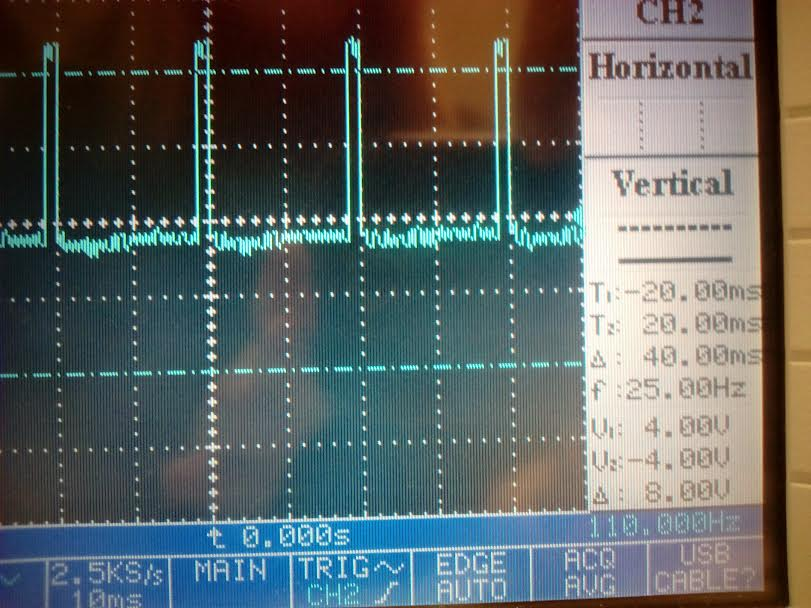
\includegraphics[width=0.5\textwidth]{images/oscillo1.jpg}
	\caption{Oscilloscope measuring APM's frequency}
	\label{oscillo1}
\end{figure}

The second experiment on the board was then made to determine how the flight controller handles the output signals during those 20$ms$. First two outputs of the APM were connected to the oscilloscope, both utilizing the Servo library to send signals of length of 2000$\mu s$. Results can be seen in figure \ref{oscillo2}.
\begin{figure}[H]
  \centering
    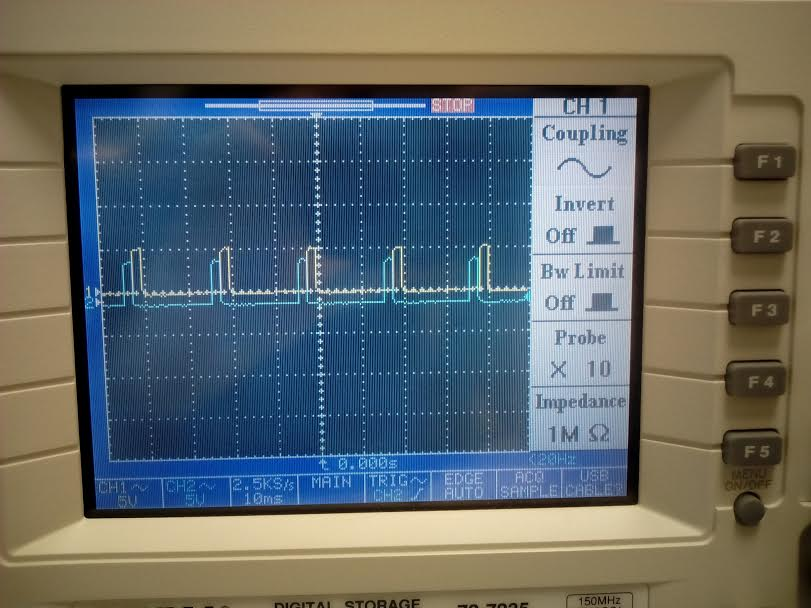
\includegraphics[width=0.5\textwidth]{images/oscillo2.jpg}
	\caption{Readings of the two output signals}
	\label{oscillo2}
\end{figure}

Then, by changing the length of the signals, two results were observed:
\begin{enumerate}
\item If the first signal is shorter than the second one, the second signal will still follow right after the first signal ends. In other words, the APM leaves no gaps between the outputs.
\item Since the board runs at the frequency of 50$Hz$ and has a period of 20$ms$, this leaves $\frac{20}{8} = 2.5ms$ maximum length for each output signal. The servo library is hard-capped at 2.4$ms$ and thus is well within the limits of the board.
\end{enumerate}

\subsection{Expected and Real Motor Performance}
The motors used in the prototype specify to be rated at $K_v$ of 980. $K_v$ is a constant describing the ration between RPM and the applied voltage and is expressed as $K_v = \frac{RPM}{V}$. Derived from this, voltage's effect on the RPM can be seen in figure \ref{KvPlot}.
\begin{figure}[H]
  \centering
    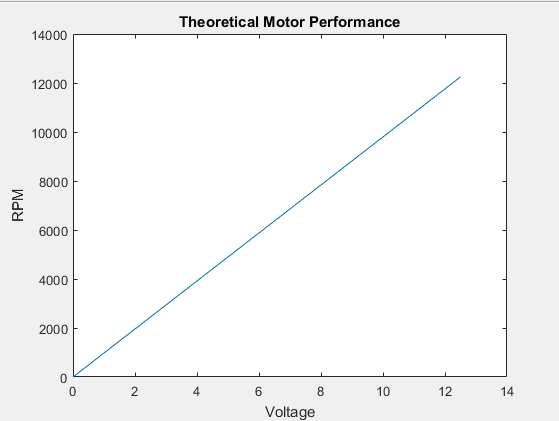
\includegraphics[width=0.8\textwidth]{images/KvPlot.png}
	\caption{Expected motor performance}
	\label{KvPlot}
\end{figure}
With a fully charged battery, the RPM is expected to be $980*11.1V = 10878 RPM$.

In order to confirm this, the actual RPM was measured using SHIMPO DT-205 digital tachometer. EXPAND WHEN WE GET THE VOLTAGE